\documentclass[border=16pt]{standalone}
\usepackage{tikz}
\usetikzlibrary{shapes,arrows.meta,positioning,calc}
\renewcommand{\familydefault}{\sfdefault}

\begin{document}
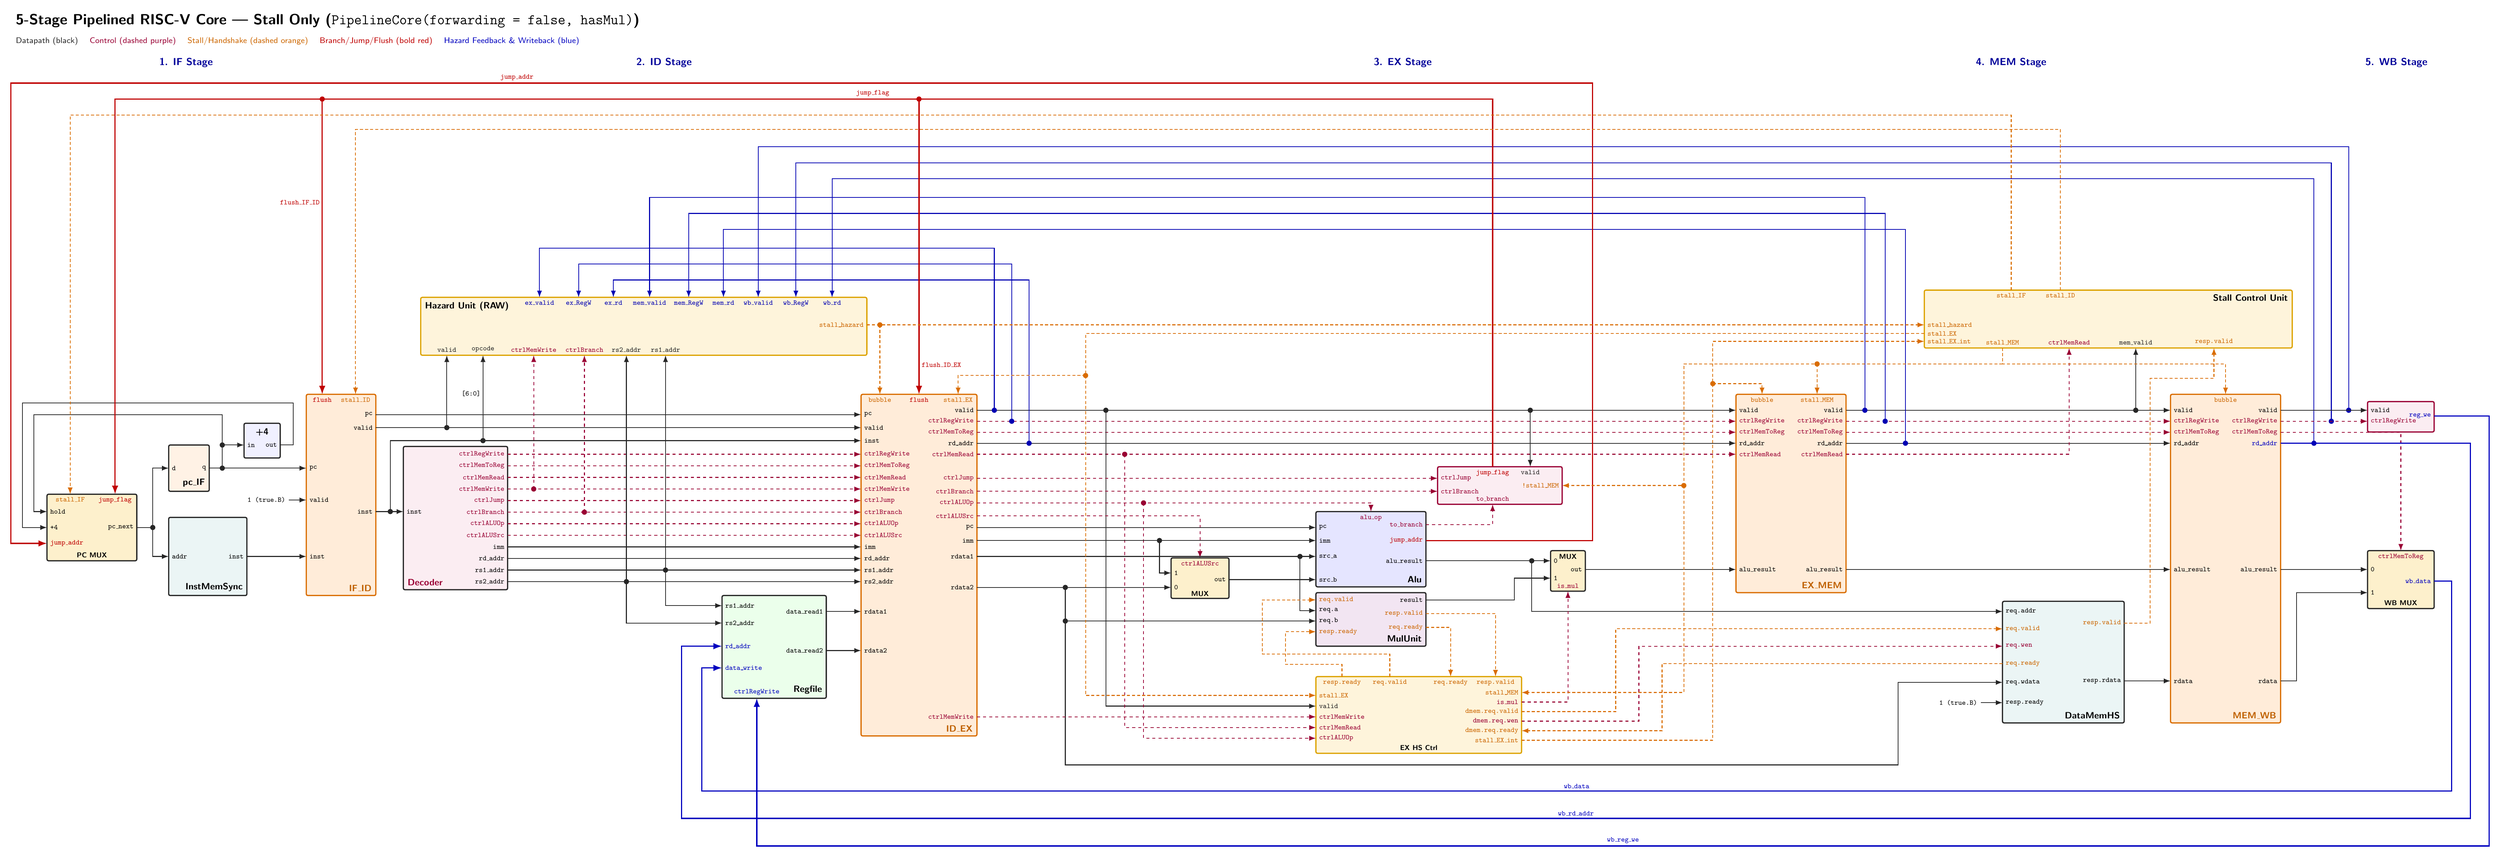
\begin{tikzpicture}[
    >=Latex,
    font=\scriptsize,
    box/.style={draw=black!85, very thick, fill=white, rounded corners=1.5pt},
    preg/.style={draw=orange!85!black, very thick, fill=orange!15, rounded corners=1.5pt},
    hbox/.style={draw=amber!90!black, very thick, fill=amber!14, rounded corners=1.5pt},
    pinL/.style={anchor=west, font=\scriptsize\ttfamily, inner sep=3pt},
    pinR/.style={anchor=east, font=\scriptsize\ttfamily, inner sep=3pt},
    pinT/.style={anchor=north, font=\scriptsize\ttfamily, inner sep=3pt},
    pinB/.style={anchor=south, font=\scriptsize\ttfamily, inner sep=3pt},
    modtitle/.style={anchor=south east, font=\small\bfseries, inner sep=4pt},
    wire/.style={->, thick, draw=black!85},
    bwire/.style={->, very thick, draw=red!75!black},
    cwire/.style={->, thick, draw=purple!80!black, dashed},
    swire/.style={->, thick, draw=orange!85!black, densely dashed},
    fbwire/.style={->, thick, draw=blue!70!black},
    wbwire/.style={->, very thick, draw=blue!75!black},
    lbl/.style={font=\scriptsize\ttfamily, inner sep=2pt},
    dot/.style={circle, fill=black!85, inner sep=1.8pt}
]
\definecolor{amber}{RGB}{245,180,0}

% =========================================================================
% Title, Legend & Stage Headers
% =========================================================================
\node[font=\Large\bfseries, anchor=west] at (-4.5, 18.75) {5-Stage Pipelined RISC-V Core --- Stall Only (\texttt{PipelineCore(forwarding = false, hasMul)})};
\node[font=\footnotesize, anchor=west] at (-4.5, 18.05) {\textcolor{black!85}{Datapath (black)} \quad \textcolor{purple!80!black}{Control (dashed purple)} \quad \textcolor{orange!80!black}{Stall/Handshake (dashed orange)} \quad \textcolor{red!75!black}{Branch/Jump/Flush (bold red)} \quad \textcolor{blue!75!black}{Hazard Feedback \& Writeback (blue)}};

\node[font=\bfseries\normalsize, text=blue!60!black] at (1.5, 17.30)  {1. IF Stage};
\node[font=\bfseries\normalsize, text=blue!60!black] at (18.0, 17.30) {2. ID Stage};
\node[font=\bfseries\normalsize, text=blue!60!black] at (43.5, 17.30) {3. EX Stage};
\node[font=\bfseries\normalsize, text=blue!60!black] at (64.5, 17.30) {4. MEM Stage};
\node[font=\bfseries\normalsize, text=blue!60!black] at (77.8, 17.30) {5. WB Stage};

% =========================================================================
% TOP CONTROL UNITS: Hazard Unit (RAW) & Stall Control Unit
% =========================================================================
% Hazard Unit (x: 9.6 .. 25.0, y: 7.20 .. 9.20) -- 9 separate top pins!
\draw[hbox] (9.6, 7.20) rectangle (25.0, 9.20);
\node[pinB, text=black!85]        at (10.50, 7.20) {valid};
\node[pinB, text=black!85]        at (11.75, 7.20) {opcode};
\node[pinB, text=purple!80!black] at (13.50, 7.20) {ctrlMemWrite};
\node[pinB, text=purple!80!black] at (15.25, 7.20) {ctrlBranch};
\node[pinB, text=black!85]        at (16.70, 7.20) {rs2\_addr};
\node[pinB, text=black!85]        at (18.05, 7.20) {rs1\_addr};
\node[pinT, text=blue!70!black]   at (13.70, 9.20) {ex\_valid};
\node[pinT, text=blue!70!black]   at (15.05, 9.20) {ex\_RegW};
\node[pinT, text=blue!70!black]   at (16.25, 9.20) {ex\_rd};
\node[pinT, text=blue!70!black]   at (17.50, 9.20) {mem\_valid};
\node[pinT, text=blue!70!black]   at (18.85, 9.20) {mem\_RegW};
\node[pinT, text=blue!70!black]   at (20.05, 9.20) {mem\_rd};
\node[pinT, text=blue!70!black]   at (21.25, 9.20) {wb\_valid};
\node[pinT, text=blue!70!black]   at (22.55, 9.20) {wb\_RegW};
\node[pinT, text=blue!70!black]   at (23.80, 9.20) {wb\_rd};
\node[pinR, text=orange!80!black] at (25.0, 8.25)  {stall\_hazard};
\node[font=\small\bfseries, anchor=north west, inner sep=4pt] at (9.6, 9.20) {Hazard Unit (RAW)};

% Stall Control Unit (x: 61.5 .. 74.2, y: 7.45 .. 9.45 -> spacious 1.60 cm corridor above EX_MEM!)
\draw[hbox] (61.5, 7.45) rectangle (74.2, 9.45);
\node[pinL, text=orange!80!black] at (61.5, 8.25) {stall\_hazard};
\node[pinL, text=orange!80!black] at (61.5, 7.95) {stall\_EX};
\node[pinL, text=orange!80!black] at (61.5, 7.68) {stall\_EX\_int};
\node[pinT, text=orange!80!black] at (64.5, 9.45) {stall\_IF};
\node[pinT, text=orange!80!black] at (66.2, 9.45) {stall\_ID};
\node[pinB, text=orange!80!black] at (64.2, 7.45) {stall\_MEM};
\node[pinB, text=purple!80!black] at (66.5, 7.45) {ctrlMemRead};
\node[pinB, text=black!85]        at (68.8, 7.45) {mem\_valid};
\node[pinB, text=orange!80!black] at (71.5, 7.45) {resp.valid};
\node[font=\small\bfseries, anchor=north east, inner sep=4pt] at (74.2, 9.45) {Stall Control Unit};

% =========================================================================
% 1. IF STAGE
% =========================================================================
\draw[box, fill=amber!20] (-3.3, 0.1) rectangle (-0.2, 2.4);
\node[pinT, text=orange!80!black] at (-2.50, 2.4) {stall\_IF};
\node[pinT, text=red!75!black]    at (-0.95, 2.4) {jump\_flag};
\node[pinL]                       at (-3.3, 1.80) {hold};
\node[pinL]                       at (-3.3, 1.25) {+4};
\node[pinL, text=red!75!black]    at (-3.3, 0.70) {jump\_addr};
\node[pinR]                       at (-0.2, 1.25) {pc\_next};
\node[font=\scriptsize\bfseries]  at (-1.75, 0.30) {PC MUX};

\draw[box, fill=orange!10] (0.9, 2.5) rectangle (2.3, 4.1);
\node[pinL] at (0.9, 3.30) {d};
\node[pinR] at (2.3, 3.30) {q};
\node[modtitle] at (2.3, 2.5) {pc\_IF};

\draw[box, fill=blue!6] (3.50, 3.65) rectangle (4.75, 4.85);
\node[pinL] at (3.50, 4.10) {in};
\node[pinR] at (4.75, 4.10) {out};
\node[font=\small\bfseries] at (4.125, 4.55) {+4};

\draw[box, fill=teal!8] (0.9, -1.1) rectangle (3.6, 1.6);
\node[pinL] at (0.9, 0.25) {addr};
\node[pinR] at (3.6, 0.25) {inst};
\node[modtitle] at (3.6, -1.1) {InstMemSync};

\draw[preg] (5.65, -1.1) rectangle (8.05, 5.85);
\node[pinT, text=red!75!black]    at (6.20, 5.85) {flush};
\node[pinT, text=orange!80!black] at (7.35, 5.85) {stall\_ID};
\node[pinL] at (5.65, 3.30) {pc};
\node[pinL] at (5.65, 2.20) {valid};
\node[pinL] at (5.65, 0.25) {inst};
\node[pinR] at (8.05, 5.15) {pc};
\node[pinR] at (8.05, 4.70) {valid};
\node[pinR] at (8.05, 1.80) {inst};
\node[modtitle, text=orange!75!black] at (8.05, -1.1) {IF\_ID};

\node[font=\scriptsize, anchor=east] at (5.05, 2.20) {\texttt{1 (true.B)}};
\draw[wire] (5.05, 2.20) -- (5.65, 2.20);

% =========================================================================
% 2. ID STAGE
% =========================================================================
\draw[box, fill=purple!7] (9.0, -0.90) rectangle (12.6, 4.05);
\node[pinL] at (9.0, 1.80) {inst};
\node[pinR, text=purple!80!black] at (12.6, 3.78) {ctrlRegWrite};
\node[pinR, text=purple!80!black] at (12.6, 3.38) {ctrlMemToReg};
\node[pinR, text=purple!80!black] at (12.6, 2.98) {ctrlMemRead};
\node[pinR, text=purple!80!black] at (12.6, 2.58) {ctrlMemWrite};
\node[pinR, text=purple!80!black] at (12.6, 2.18) {ctrlJump};
\node[pinR, text=purple!80!black] at (12.6, 1.78) {ctrlBranch};
\node[pinR, text=purple!80!black] at (12.6, 1.38) {ctrlALUOp};
\node[pinR, text=purple!80!black] at (12.6, 0.98) {ctrlALUSrc};
\node[pinR]                       at (12.6, 0.58) {imm};
\node[pinR]                       at (12.6, 0.18) {rd\_addr};
\node[pinR]                       at (12.6,-0.22) {rs1\_addr};
\node[pinR]                       at (12.6,-0.62) {rs2\_addr};
\node[modtitle, anchor=south west, text=purple!80!black] at (9.0, -0.90) {Decoder};

\draw[box, fill=green!8] (20.0, -4.65) rectangle (23.6, -1.10);
\node[pinL]                       at (20.0, -1.45) {rs1\_addr};
\node[pinL]                       at (20.0, -2.05) {rs2\_addr};
\node[pinL, text=blue!75!black]   at (20.0, -2.85) {rd\_addr};
\node[pinL, text=blue!75!black]   at (20.0, -3.60) {data\_write};
\node[pinB, text=blue!75!black]   at (21.2, -4.65) {ctrlRegWrite};
\node[pinR]                       at (23.6, -1.65) {data\_read1};
\node[pinR]                       at (23.6, -3.00) {data\_read2};
\node[modtitle] at (23.6, -4.65) {Regfile};

% ID_EX Pipeline Register (x: 24.8 .. 28.8, y: -5.95 .. 5.85 -> wide 4.0 cm, full names on BOTH sides!)
\draw[preg] (24.8, -5.95) rectangle (28.8, 5.85);
\node[pinT, text=orange!80!black] at (25.45, 5.85) {bubble};
\node[pinT, text=red!75!black]    at (26.80, 5.85) {flush};
\node[pinT, text=orange!80!black] at (28.15, 5.85) {stall\_EX};
% Left pins (full names!)
\node[pinL] at (24.8, 5.15) {pc};
\node[pinL] at (24.8, 4.70) {valid};
\node[pinL] at (24.8, 4.25) {inst};
\node[pinL, text=purple!80!black] at (24.8, 3.78) {ctrlRegWrite};
\node[pinL, text=purple!80!black] at (24.8, 3.38) {ctrlMemToReg};
\node[pinL, text=purple!80!black] at (24.8, 2.98) {ctrlMemRead};
\node[pinL, text=purple!80!black] at (24.8, 2.58) {ctrlMemWrite};
\node[pinL, text=purple!80!black] at (24.8, 2.18) {ctrlJump};
\node[pinL, text=purple!80!black] at (24.8, 1.78) {ctrlBranch};
\node[pinL, text=purple!80!black] at (24.8, 1.38) {ctrlALUOp};
\node[pinL, text=purple!80!black] at (24.8, 0.98) {ctrlALUSrc};
\node[pinL] at (24.8, 0.58)  {imm};
\node[pinL] at (24.8, 0.18)  {rd\_addr};
\node[pinL] at (24.8,-0.22)  {rs1\_addr};
\node[pinL] at (24.8,-0.62)  {rs2\_addr};
\node[pinL] at (24.8,-1.65)  {rdata1};
\node[pinL] at (24.8,-3.00)  {rdata2};
% Right pins (full names!)
\node[pinR]                       at (28.8, 5.30) {valid};
\node[pinR, text=purple!80!black] at (28.8, 4.92) {ctrlRegWrite};
\node[pinR, text=purple!80!black] at (28.8, 4.54) {ctrlMemToReg};
\node[pinR]                       at (28.8, 4.16) {rd\_addr};
\node[pinR, text=purple!80!black] at (28.8, 3.78) {ctrlMemRead};
\node[pinR, text=purple!80!black] at (28.8, 2.95) {ctrlJump};
\node[pinR, text=purple!80!black] at (28.8, 2.50) {ctrlBranch};
\node[pinR, text=purple!80!black] at (28.8, 2.10) {ctrlALUOp};
\node[pinR, text=purple!80!black] at (28.8, 1.65) {ctrlALUSrc};
\node[pinR]                       at (28.8, 1.25) {pc};
\node[pinR]                       at (28.8, 0.80) {imm};
\node[pinR]                       at (28.8, 0.25) {rdata1};
\node[pinR]                       at (28.8,-0.82) {rdata2};
\node[pinR, text=purple!80!black] at (28.8,-5.29) {ctrlMemWrite};
\node[modtitle, text=orange!75!black] at (28.8, -5.95) {ID\_EX};

% =========================================================================
% 3. EX STAGE
% =========================================================================
% ALUSrc MUX (x: 35.5 .. 37.5, y: -1.20 .. 0.20 -> generous clearance!)
\draw[box, fill=amber!20] (35.5, -1.20) rectangle (37.5, 0.20);
\node[pinT, text=purple!80!black] at (36.50, 0.20) {ctrlALUSrc};
\node[pinL] at (35.5, -0.32) {1};
\node[pinL] at (35.5, -0.82) {0};
\node[pinR] at (37.5, -0.55) {out};
\node[font=\scriptsize\bfseries] at (36.50, -1.04) {MUX};

% Alu (x: 40.5 .. 44.3, y: -0.80 .. 1.80)
\draw[box, fill=blue!10] (40.5, -0.80) rectangle (44.3, 1.80);
\node[pinT, text=purple!80!black] at (42.40, 1.80) {alu\_op};
\node[pinL] at (40.5, 1.25) {pc};
\node[pinL] at (40.5, 0.80) {imm};
\node[pinL] at (40.5, 0.25) {src\_a};
\node[pinL] at (40.5,-0.55) {src\_b};
\node[pinR, text=purple!80!black] at (44.3, 1.35) {to\_branch};
\node[pinR, text=red!75!black]    at (44.3, 0.80) {jump\_addr};
\node[pinR]                       at (44.3, 0.10) {alu\_result};
\node[modtitle] at (44.3, -0.80) {Alu};

% Branch / Jump Gate (x: 44.7 .. 49.0, y: 2.05 .. 3.35)
\draw[box, fill=purple!7, draw=purple!80!black] (44.7, 2.05) rectangle (49.0, 3.35);
\node[pinL, text=purple!80!black] at (44.7, 2.95) {ctrlJump};
\node[pinL, text=purple!80!black] at (44.7, 2.50) {ctrlBranch};
\node[pinB, text=purple!80!black] at (46.60, 2.05) {to\_branch};
\node[pinT, text=red!75!black]    at (46.60, 3.35) {jump\_flag};
\node[pinT, text=black!85]        at (47.90, 3.35) {valid};
\node[pinR, text=orange!80!black] at (49.0, 2.70) {!stall\_MEM};

% MulUnit (x: 40.5 .. 44.3, y: -2.85 .. -1.00)
\draw[box, fill=violet!10] (40.5, -2.85) rectangle (44.3, -1.00);
\node[pinL, text=orange!80!black] at (40.5, -1.25) {req.valid};
\node[pinL]                       at (40.5, -1.62) {req.a};
\node[pinL]                       at (40.5, -1.98) {req.b};
\node[pinL, text=orange!80!black] at (40.5, -2.35) {resp.ready};
\node[pinR]                       at (44.3, -1.25) {result};
\node[pinR, text=orange!80!black] at (44.3, -1.72) {resp.valid};
\node[pinR, text=orange!80!black] at (44.3, -2.20) {req.ready};
\node[modtitle] at (44.3, -2.85) {MulUnit};

% EX Result MUX (x: 48.6 .. 49.8, y: -0.95 .. 0.45)
\draw[box, fill=amber!20] (48.6, -0.95) rectangle (49.8, 0.45);
\node[pinB, text=purple!80!black] at (49.20, -0.95) {is\_mul};
\node[pinL] at (48.6,  0.10) {0};
\node[pinL] at (48.6, -0.50) {1};
\node[pinR] at (49.8, -0.20) {out};
\node[font=\scriptsize\bfseries] at (49.20, 0.25) {MUX};

% EX HS Ctrl (x: 40.5 .. 47.6, y: -6.55 .. -3.90 -> nested zero-crossing Mul handshake!)
\draw[hbox] (40.5, -6.55) rectangle (47.6, -3.90);
\node[pinL, text=orange!80!black] at (40.5, -4.55) {stall\_EX};
\node[pinL, text=black!85]        at (40.5, -4.92) {valid};
\node[pinL, text=purple!80!black] at (40.5, -5.29) {ctrlMemWrite};
\node[pinL, text=purple!80!black] at (40.5, -5.66) {ctrlMemRead};
\node[pinL, text=purple!80!black] at (40.5, -6.03) {ctrlALUOp};
\node[pinT, text=orange!80!black] at (41.40,-3.90) {resp.ready};
\node[pinT, text=orange!80!black] at (43.05,-3.90) {req.valid};
\node[pinT, text=orange!80!black] at (45.15,-3.90) {req.ready};
\node[pinT, text=orange!80!black] at (46.70,-3.90) {resp.valid};
\node[pinR, text=orange!80!black] at (47.6, -4.45) {stall\_MEM};
\node[pinR, text=purple!80!black] at (47.6, -4.78) {is\_mul};
\node[pinR, text=orange!80!black] at (47.6, -5.11) {dmem.req.valid};
\node[pinR, text=purple!80!black] at (47.6, -5.44) {dmem.req.wen};
\node[pinR, text=orange!80!black] at (47.6, -5.77) {dmem.req.ready};
\node[pinR, text=orange!80!black] at (47.6, -6.10) {stall\_EX\_int};
\node[font=\scriptsize\bfseries, anchor=south, inner sep=3pt] at (44.05, -6.55) {EX HS Ctrl};

% =========================================================================
% 4. MEM STAGE
% =========================================================================
% EX_MEM Pipeline Register (x: 55.0 .. 58.8 -> wide 3.8 cm, full names!)
\draw[preg] (55.0, -1.00) rectangle (58.8, 5.85);
\node[pinT, text=orange!80!black] at (55.90, 5.85) {bubble};
\node[pinT, text=orange!80!black] at (57.80, 5.85) {stall\_MEM};
\node[pinL]                       at (55.0, 5.30) {valid};
\node[pinL, text=purple!80!black] at (55.0, 4.92) {ctrlRegWrite};
\node[pinL, text=purple!80!black] at (55.0, 4.54) {ctrlMemToReg};
\node[pinL]                       at (55.0, 4.16) {rd\_addr};
\node[pinL, text=purple!80!black] at (55.0, 3.78) {ctrlMemRead};
\node[pinL]                       at (55.0,-0.20) {alu\_result};
\node[pinR]                       at (58.8, 5.30) {valid};
\node[pinR, text=purple!80!black] at (58.8, 4.92) {ctrlRegWrite};
\node[pinR, text=purple!80!black] at (58.8, 4.54) {ctrlMemToReg};
\node[pinR]                       at (58.8, 4.16) {rd\_addr};
\node[pinR, text=purple!80!black] at (58.8, 3.78) {ctrlMemRead};
\node[pinR]                       at (58.8,-0.20) {alu\_result};
\node[modtitle, text=orange!75!black] at (58.8, -1.00) {EX\_MEM};

% DataMemHS (x: 64.2 .. 68.4, y: -5.50 .. -1.30)
\draw[box, fill=teal!8] (64.2, -5.50) rectangle (68.4, -1.30);
\node[pinL]                       at (64.2, -1.65) {req.addr};
\node[pinL, text=orange!80!black] at (64.2, -2.25) {req.valid};
\node[pinL, text=purple!80!black] at (64.2, -2.85) {req.wen};
\node[pinL, text=orange!80!black] at (64.2, -3.45) {req.ready};
\node[pinL]                       at (64.2, -4.10) {req.wdata};
\node[pinL]                       at (64.2, -4.80) {resp.ready};
\node[pinR, text=orange!80!black] at (68.4, -2.05) {resp.valid};
\node[pinR]                       at (68.4, -4.05) {resp.rdata};
\node[modtitle] at (68.4, -5.50) {DataMemHS};

\node[font=\scriptsize, anchor=east] at (63.45, -4.80) {\texttt{1 (true.B)}};
\draw[wire] (63.45, -4.80) -- (64.2, -4.80);

% MEM_WB Pipeline Register (x: 70.0 .. 73.8 -> wide 3.8 cm, full names!)
\draw[preg] (70.0, -5.50) rectangle (73.8, 5.85);
\node[pinT, text=orange!80!black] at (71.90, 5.85) {bubble};
\node[pinL]                       at (70.0, 5.30) {valid};
\node[pinL, text=purple!80!black] at (70.0, 4.92) {ctrlRegWrite};
\node[pinL, text=purple!80!black] at (70.0, 4.54) {ctrlMemToReg};
\node[pinL]                       at (70.0, 4.16) {rd\_addr};
\node[pinL]                       at (70.0,-0.20) {alu\_result};
\node[pinL]                       at (70.0,-4.05) {rdata};
\node[pinR]                       at (73.8, 5.30) {valid};
\node[pinR, text=purple!80!black] at (73.8, 4.92) {ctrlRegWrite};
\node[pinR, text=purple!80!black] at (73.8, 4.54) {ctrlMemToReg};
\node[pinR, text=blue!75!black]   at (73.8, 4.16) {rd\_addr};
\node[pinR]                       at (73.8,-0.20) {alu\_result};
\node[pinR]                       at (73.8,-4.05) {rdata};
\node[modtitle, text=orange!75!black] at (73.8, -5.50) {MEM\_WB};

% =========================================================================
% 5. WB STAGE
% =========================================================================
\draw[box, fill=purple!7, draw=purple!80!black] (76.8, 4.55) rectangle (79.1, 5.60);
\node[pinL]                       at (76.8, 5.30) {valid};
\node[pinL, text=purple!80!black] at (76.8, 4.92) {ctrlRegWrite};
\node[pinR, text=blue!75!black]   at (79.1, 5.10) {reg\_we};

\draw[box, fill=amber!20] (76.8, -1.55) rectangle (79.1, 0.45);
\node[pinT, text=purple!80!black] at (77.95, 0.45) {ctrlMemToReg};
\node[pinL]                       at (76.8, -0.20) {0};
\node[pinL]                       at (76.8, -1.00) {1};
\node[pinR, text=blue!75!black]   at (79.1, -0.60) {wb\_data};
\node[font=\scriptsize\bfseries]  at (77.95, -1.35) {WB MUX};

% =========================================================================
% WIRES & CONNECTIONS (ZERO shared wires across different signals!)
% =========================================================================
% --- 1. IF Stage ---
\draw[wire] (-0.2, 1.25) -- (0.35, 1.25) |- (0.9, 3.30);
\node[dot] at (0.35, 1.25) {};
\draw[wire] (0.35, 1.25) |- (0.9, 0.25);

\draw[wire] (2.3, 3.30) -- (5.65, 3.30);
\node[dot] at (2.75, 3.30) {};
\draw[wire] (2.75, 3.30) -- (2.75, 4.10) -- (3.50, 4.10);
\node[dot] at (2.75, 4.10) {};
\draw[wire] (2.75, 4.10) -- (2.75, 5.15) -- (-3.75, 5.15) |- (-3.3, 1.80);
\draw[wire] (4.75, 4.10) -- (5.20, 4.10) -- (5.20, 5.55) -- (-4.15, 5.55) |- (-3.3, 1.25);
\draw[wire] (3.6, 0.25) -- (5.65, 0.25);

% --- 2. IF_ID -> ID Stage ---
\draw[wire] (8.05, 5.15) -- (24.8, 5.15);
\draw[wire] (8.05, 4.70) -- (24.8, 4.70);
\node[dot] at (10.50, 4.70) {};
\draw[wire] (10.50, 4.70) -- (10.50, 7.20);

\draw[wire] (8.05, 1.80) -- (9.0, 1.80);
\node[dot] at (8.55, 1.80) {};
\draw[wire] (8.55, 1.80) -- (8.55, 4.25) -- (24.8, 4.25);
\node[dot] at (11.75, 4.25) {};
\draw[wire] (11.75, 4.25) -- node[lbl, left, pos=0.55]{\texttt{[6:0]}} (11.75, 7.20);

\draw[cwire] (12.6, 3.78) -- (24.8, 3.78);
\draw[cwire] (12.6, 3.38) -- (24.8, 3.38);
\draw[cwire] (12.6, 2.98) -- (24.8, 2.98);
\draw[cwire] (12.6, 2.58) -- (24.8, 2.58);
\node[dot, fill=purple!80!black] at (13.50, 2.58) {};
\draw[cwire] (13.50, 2.58) -- (13.50, 7.20);
\draw[cwire] (12.6, 2.18) -- (24.8, 2.18);
\draw[cwire] (12.6, 1.78) -- (24.8, 1.78);
\node[dot, fill=purple!80!black] at (15.25, 1.78) {};
\draw[cwire] (15.25, 1.78) -- (15.25, 7.20);
\draw[cwire] (12.6, 1.38) -- (24.8, 1.38);
\draw[cwire] (12.6, 0.98) -- (24.8, 0.98);
\draw[wire]  (12.6, 0.58) -- (24.8, 0.58);
\draw[wire]  (12.6, 0.18) -- (24.8, 0.18);

\draw[wire] (12.6, -0.22) -- (24.8, -0.22);
\node[dot] at (18.05, -0.22) {};
\draw[wire] (18.05, -0.22) -- (18.05, 7.20);
\draw[wire] (18.05, -0.22) -- (18.05, -1.45) -- (20.0, -1.45);

\draw[wire] (12.6, -0.62) -- (24.8, -0.62);
\node[dot] at (16.70, -0.62) {};
\draw[wire] (16.70, -0.62) -- (16.70, 7.20);
\draw[wire] (16.70, -0.62) -- (16.70, -2.05) -- (20.0, -2.05);

\draw[wire] (23.6, -1.65) -- (24.8, -1.65);
\draw[wire] (23.6, -3.00) -- (24.8, -3.00);

% --- 3. ID_EX -> EX Stage (10 strictly separate vertical columns!) ---
\draw[wire]  (28.8, 5.30) -- (55.0, 5.30);
\draw[cwire] (28.8, 4.92) -- (55.0, 4.92);
\draw[cwire] (28.8, 4.54) -- (55.0, 4.54);
\draw[wire]  (28.8, 4.16) -- (55.0, 4.16);
\draw[cwire] (28.8, 3.78) -- (55.0, 3.78);

% 3 SEPARATE Hazard Unit feedback wires from ID_EX (0.55 cm vertical pitch!)
\node[dot, fill=blue!70!black] at (29.40, 5.30) {};
\draw[fbwire] (29.40, 5.30) -- (29.40, 10.90) -| (13.70, 9.20);
\node[dot, fill=blue!70!black] at (30.00, 4.92) {};
\draw[fbwire] (30.00, 4.92) -- (30.00, 10.35) -| (15.05, 9.20);
\node[dot, fill=blue!70!black] at (30.60, 4.16) {};
\draw[fbwire] (30.60, 4.16) -- (30.60,  9.80) -| (16.25, 9.20);

\node[dot] at (47.90, 5.30) {};
\draw[wire] (47.90, 5.30) -- (47.90, 3.35);

\node[dot] at (33.25, 5.30) {};
\draw[wire]  (33.25, 5.30) -- (33.25, -4.92) -- (40.5, -4.92);
\node[dot, fill=purple!80!black] at (33.90, 3.78) {};
\draw[cwire] (33.90, 3.78) -- (33.90, -5.66) -- (40.5, -5.66);
\node[dot, fill=purple!80!black] at (34.55, 2.10) {};
\draw[cwire] (34.55, 2.10) -- (34.55, -6.03) -- (40.5, -6.03);

\draw[cwire] (28.8, 2.95) -- (44.7, 2.95);
\draw[cwire] (28.8, 2.50) -- (44.7, 2.50);
\draw[cwire] (28.8, 2.10) -| (42.40, 1.80);
\draw[cwire] (28.8, 1.65) -| (36.50, 0.20);

\draw[wire] (28.8, 1.25) -- (40.5, 1.25);
\draw[wire] (28.8, 0.80) -- (40.5, 0.80);
\node[dot] at (35.10, 0.80) {};
\draw[wire] (35.10, 0.80) |- (35.5, -0.32);

\draw[wire] (28.8, 0.25) -- (40.5, 0.25);
\node[dot] at (39.95, 0.25) {};
\draw[wire] (39.95, 0.25) |- (40.5, -1.62);

\draw[wire] (28.8, -0.82) -- (35.5, -0.82);
\node[dot] at (31.85, -0.82) {};
\draw[wire] (31.85, -0.82) |- (40.5, -1.98);
\node[dot] at (31.85, -1.98) {};
\draw[wire] (31.85, -1.98) -- (31.85, -6.95) -- (60.60, -6.95) |- (64.2, -4.10);

\draw[cwire] (28.8, -5.29) -- (40.5, -5.29);
\draw[wire] (37.5, -0.55) -- (40.5, -0.55);

% Alu -> Branch/Jump, EX Result MUX, DataMemHS
\draw[cwire] (44.3, 1.35) -| (46.60, 2.05);
\draw[wire]  (44.3, 0.10) -- (48.6, 0.10);
\node[dot] at (47.95, 0.10) {};
\draw[wire]  (47.95, 0.10) |- (64.2, -1.65);

% MulUnit <-> EX HS Ctrl (4 NON-CROSSING nested/L-turn handshake wires!)
\draw[wire]  (44.3, -1.25) -- (47.35, -1.25) |- (48.6, -0.50);
\draw[swire] (44.3, -1.72) -- (46.70, -1.72) -- (46.70, -3.90);
\draw[swire] (44.3, -2.20) -- (45.15, -2.20) -- (45.15, -3.90);
\draw[swire] (41.40, -3.90) -- (41.40, -3.48) -- (39.45, -3.48) -- (39.45, -2.35) -- (40.5, -2.35);
\draw[swire] (43.05, -3.90) -- (43.05, -3.12) -- (38.65, -3.12) -- (38.65, -1.25) -- (40.5, -1.25);

\draw[cwire] (47.6, -4.78) -| (49.20, -0.95);
\draw[swire] (47.6, -5.11) -- (50.85, -5.11) |- (64.2, -2.25);
\draw[cwire] (47.6, -5.44) -- (51.65, -5.44) |- (64.2, -2.85);
\draw[swire] (64.2, -3.45) -| (52.45, -5.77) -- (47.6, -5.77);

\draw[wire] (49.8, -0.20) -- (55.0, -0.20);

% --- 4. EX_MEM -> MEM_WB & Stall Unit & Hazard Unit (3 SEPARATE EX_MEM wires!) ---
\draw[wire]  (58.8, 5.30) -- (70.0, 5.30);
\draw[cwire] (58.8, 4.92) -- (70.0, 4.92);
\draw[cwire] (58.8, 4.54) -- (70.0, 4.54);
\draw[wire]  (58.8, 4.16) -- (70.0, 4.16);
\draw[wire]  (58.8,-0.20) -- (70.0,-0.20);

\draw[cwire] (58.8, 3.78) -- (66.5, 3.78) -- (66.5, 7.45);
\node[dot] at (68.8, 5.30) {};
\draw[wire] (68.8, 5.30) -- (68.8, 7.45);
\draw[swire] (68.4, -2.05) -- (69.30, -2.05) -- (69.30, 6.40) -- (71.5, 6.40) -- (71.5, 7.45);
\draw[wire]  (68.4, -4.05) -- (70.0, -4.05);

% 3 SEPARATE EX_MEM -> Hazard Unit feedback wires (0.55 cm vertical pitch!)
\node[dot, fill=blue!70!black] at (59.45, 5.30) {};
\draw[fbwire] (59.45, 5.30) -- (59.45, 12.65) -| (17.50, 9.20);
\node[dot, fill=blue!70!black] at (60.15, 4.92) {};
\draw[fbwire] (60.15, 4.92) -- (60.15, 12.10) -| (18.85, 9.20);
\node[dot, fill=blue!70!black] at (60.85, 4.16) {};
\draw[fbwire] (60.85, 4.16) -- (60.85, 11.55) -| (20.05, 9.20);

% 3 SEPARATE MEM_WB -> Hazard Unit feedback wires (0.55 cm vertical pitch!)
\node[dot, fill=blue!70!black] at (74.95, 4.16) {};
\draw[fbwire] (74.95, 4.16) -- (74.95, 13.30) -| (23.80, 9.20);
\node[dot, fill=blue!70!black] at (75.55, 4.92) {};
\draw[fbwire] (75.55, 4.92) -- (75.55, 13.85) -| (22.55, 9.20);
\node[dot, fill=blue!70!black] at (76.15, 5.30) {};
\draw[fbwire] (76.15, 5.30) -- (76.15, 14.40) -| (21.25, 9.20);

% --- 5. MEM_WB -> WB Stage & Bottom Writeback ---
\draw[wire]  (73.8, 5.30) -- (76.8, 5.30);
\draw[cwire] (73.8, 4.92) -- (76.8, 4.92);
\draw[cwire] (73.8, 4.54) -| (77.95, 0.45);
\draw[wire]  (73.8,-0.20) -- (76.8,-0.20);
\draw[wire]  (73.8,-4.05) -- (74.35,-4.05) |- (76.8,-1.00);

% 3 SEPARATE Bottom Writeback lines (0.95 cm vertical pitch!)
\draw[wbwire] (79.1, -0.60) -- (79.70, -0.60) -- (79.70, -7.85) -- node[lbl, text=blue!75!black, above, pos=0.50]{\texttt{wb\_data}} (19.30, -7.85) |- (20.0, -3.60);
\draw[wbwire] (73.8,  4.16) -- (80.35,  4.16) -- (80.35, -8.80) -- node[lbl, text=blue!75!black, above, pos=0.50]{\texttt{wb\_rd\_addr}} (18.60, -8.80) |- (20.0, -2.85);
\draw[wbwire] (79.1,  5.10) -- (81.00,  5.10) -- (81.00, -9.75) -- node[lbl, text=blue!75!black, above, pos=0.50]{\texttt{wb\_reg\_we}} (21.20, -9.75) -- (21.2, -4.65);

% --- 6. Top Branch/Jump Redirect ---
\draw[bwire] (44.3, 0.80) -- (50.05, 0.80) -- (50.05, 16.60) -- node[lbl, text=red!75!black, above, pos=0.68]{\texttt{jump\_addr}} (-4.55, 16.60) |- (-3.3, 0.70);
\draw[bwire] (46.60, 3.35) -- (46.60, 16.05) -- node[lbl, text=red!75!black, above, pos=0.45]{\texttt{jump\_flag}} (-0.95, 16.05) -- (-0.95, 2.4);
\node[dot, fill=red!75!black] at (26.80, 16.05) {};
\draw[bwire] (26.80, 16.05) -- node[lbl, text=red!75!black, right, pos=0.90]{\texttt{flush\_ID\_EX}} (26.80, 5.85);
\node[dot, fill=red!75!black] at (6.20, 16.05) {};
\draw[bwire] (6.20, 16.05) -- node[lbl, text=red!75!black, left, pos=0.35]{\texttt{flush\_IF\_ID}} (6.20, 5.85);

% --- 7. Stall Cascade ---
\draw[swire] (25.0, 8.25) -- (61.5, 8.25);
\node[dot, fill=orange!85!black] at (25.45, 8.25) {};
\draw[swire] (25.45, 8.25) -- (25.45, 5.85);

\draw[swire] (64.5, 9.45) -- (64.5, 15.50) -- (-2.50, 15.50) -- (-2.50, 2.4);
\draw[swire] (66.2, 9.45) -- (66.2, 15.00) -- (7.35, 15.00) -- (7.35, 5.85);

\draw[swire] (61.5, 7.95) -- (32.55, 7.95) -- (32.55, 6.50) -- (28.15, 6.50) -- (28.15, 5.85);
\node[dot, fill=orange!85!black] at (32.55, 6.50) {};
\draw[swire] (32.55, 6.50) -- (32.55, -4.55) -- (40.5, -4.55);

% stall_EX_int (x=54.20 -> lower track y=6.22 into EX_MEM.bubble 55.90 & Stall Unit 61.5, 7.68)
\draw[swire] (47.6, -6.10) -- (54.20, -6.10) -- (54.20, 7.68) -- (61.5, 7.68);
\node[dot, fill=orange!85!black] at (54.20, 6.22) {};
\draw[swire] (54.20, 6.22) -| (55.90, 5.85);

% stall_MEM (x=64.2 -> upper track y=6.90 -> EX_MEM.stall_MEM 57.80, MEM_WB.bubble 71.90, & EX !stall_MEM at x=53.20)
\draw[swire] (64.2, 7.45) -- (64.2, 6.90) -- (71.90, 6.90) -- (71.90, 5.85);
\node[dot, fill=orange!85!black] at (57.80, 6.90) {};
\draw[swire] (57.80, 6.90) -- (57.80, 5.85);
\draw[swire] (64.2, 6.90) -- (53.20, 6.90) -- (53.20, 2.70) -- (49.0, 2.70);
\node[dot, fill=orange!85!black] at (53.20, 2.70) {};
\draw[swire] (53.20, 2.70) -- (53.20, -4.45) -- (47.6, -4.45);

\end{tikzpicture}
\end{document}
